%TODO: Erw�hnen, welche balancierten Subsets genutzt wurden

\chapter{Language identification} \label{chap:langid}
Singing language identification is the task of automatically determining the language of a sung recording. For this task, two algorithms were developed: One based on i-Vector extraction, and one based on the statistics of phoneme posteriorgrams. They will be described in detail in this section.\\
In both cases, the \textit{NIST2003LRE} and \textit{OGIMultilang} corpora were used for testing the algorithms on speech, and the \textit{YTAcap} data set was used for singing (see chapter \ref{chap:Data}).

\section{Language identification in singing using i-vectors}
%known speakers - unknown speakers - whole documents


As described in section \ref{sec:tech_ivector}, i-Vector extraction is a feature dimension reduction algorithm that was originally developed for speaker recognition, but has since then been employed successfully for other tasks, including language identification. After the publication of this approach for i-Vector extraction for singing language identification, they also became used for other MIR tasks, such as artist recognition and similarity calculation \cite{eghbal-zadeh1} \cite{eghbal-zadeh2}.

\section{Proposed system}
\label{sec:system}
Figure \ref{fig:lid_ivectors} shows a rough overview over the i-vector classification system. 
%\begin{figure}[ht]
%\centerline{\includegraphics[scale=0.3]%{overview.png}}
%\caption{\label{fig:overview}{\it Overview of the steps of our classification system.}}
%\end{figure}
\begin{figure*}
	\begin{center}
		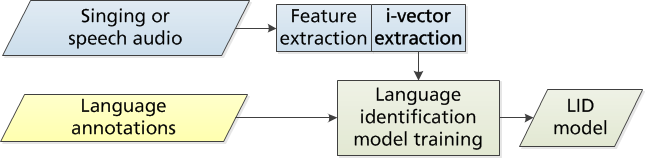
\includegraphics[width=.8\textwidth]{images/lid_ivectors.png}
		\caption{Overview of the process for language identification using i-vector extraction.}
		\label{fig:lid_ivectors}
	\end{center}
\end{figure*}

A number of features were extracted from each audio file. Table \ref{tab:configs} shows an overview over the various configurations used in training.
\begin{table*}[h!tbp]
\scriptsize
  \caption{{ Feature configurations used in training.}}
  \begin{center}
     \begin{tabular}{|c|c|c|}\hline
     Name & Description & Dimensions \\ \hline
      MFCC  & MFCC, 20 coefficients & 20 \\
      MFCCDELTA  & MFCC, 20 coefficients, deltas and double deltas & 60 \\
      MFCCDELTASDC  & MFCCDELTA+SDC & 117 \\
      SDC  & SDC with configuration $7-1-3-7$ & 91 \\
      RASTA-PLP & PLP with RASTA processing, model order 13 with deltas and double deltas & 39 \\
      RASTA-PLP36  & PLP with RASTA processing, model order 36 with deltas and double deltas  & 96 \\
      PLP  & PLP without RASTA processing, model order 13 deltas and double deltas  & 39 \\
      COMB & PLP+MFCCDELTA & 99 \\ \hline
    \end{tabular}
  \end{center}
  \label{tab:configs}
\end{table*}

For classification, Multi-Layer Perceptrons (MLPs) and Support Vector Machines (SVMs) were tested. The MLPs were fixed at three layers, with the middle layer having a dimension of 256. Additional layers did not seem to improve the result. A larger middle layer only improved it slightly. The SVM parameters were determined using a grid-search. For each of those classifiers and data sets, all combinations of the features listed in table \ref{tab:configs} were tested directly and with i-vector processing. All results were obtained using five-fold cross validation. \\


\subsection{Experiments with known speakers}
In the first experiment, MLP and SVM models were trained on randomly selected folds of the training data sets. This means that recordings by the same speaker are spread out between the training and test data sets. In theory, i-vectors could be particularly susceptible to capturing speaker characteristics instead of language characteristics, leading to evaluation results that may not be representative of results for unknown speakers. However, this effect is often ignored in literature \cite{Martin2010}, and an argument can be made that partially training models on speaker properties is realistic for some use cases (i.e. when many of the expected speakers for each language are already known).\\

\begin{figure}[h]
       \centering
      \begin{subfigure}[b]{0.3\textwidth}
                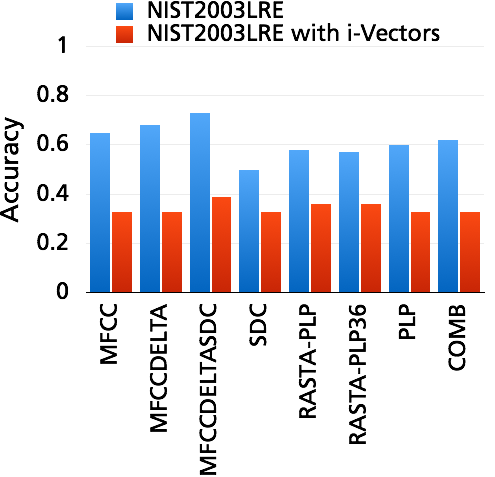
\includegraphics[width=\textwidth]{images/lid_exp1_nist.png}
                \caption{NIST2003LRE}
                \label{fig:lid_exp1_nist}
        \end{subfigure}%
        \begin{subfigure}[b]{0.3\textwidth}
                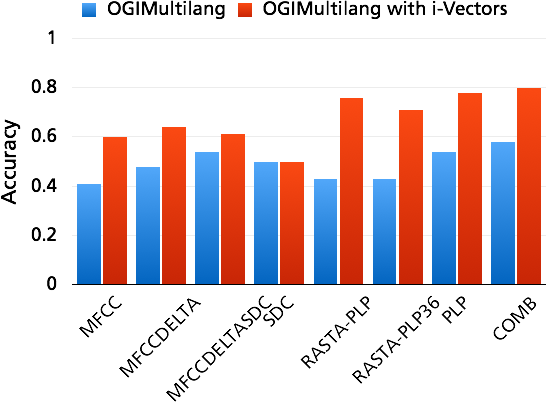
\includegraphics[width=\textwidth]{images/lid_exp1_ogi.png}
                \caption{OGIMultilang}
                \label{fig:exp1_ogi}
        \end{subfigure}
                \begin{subfigure}[b]{0.3\textwidth}
                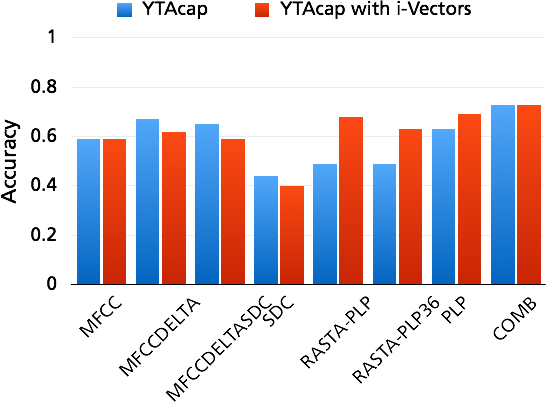
\includegraphics[width=\textwidth]{images/lid_exp1_yt.png}
                \caption{YTAcap}
                \label{fig:exp1_yt}
        \end{subfigure}
        \caption{Results using MLP models on all three language identification data sets, with or without i-vector processing.}\label{fig:lid_exp1}
\end{figure}

The results for the MLP training on the \textit{NIST2003LRE}, \textit{OGIMultilang}, and \textit{YTAcap} data sets are shown in figure \ref{fig:lid_exp1}. \\
As shown in figure \ref{fig:lid_exp1_nist}, the MLP did not produce good results on the \textit{NIST2003LRE} database for any of the feature combinations. \textit{NIST2003LRE} is the smallest of the data sets by a large margin. Since a relatively high-dimensional model was used, this is probably a case of overtraining. The i-vector processing step reduces the training data even further, thus aggravating the problem.\\
The \textit{OGIMultilang} data set contains roughly 4 times as much data as the \textit{NIST2003LRE} set. With enough data, training an MLP classifier works a lot better. Without i-vector processing, this approach still only reach about 52\% accuracy. i-Vector extraction improves the system massively. The best feature configurations are RASTA-PLP (82\%), PLP (80\%), and COMB (80\%).\\
As with all other experiments, the task becomes harder when attempted on singing data. The results on the \textit{YTAcap} data set are somewhat worse than those on \textit{OGIMultilang}, even though they contain a similar amount of data. The best result without i-vector extraction is still obtained using the COMB feature configuration at 56\%. Similar to the \textit{OGIMultilang} experiment, i-vector extraction yields a large improvement. COMB remains the best configuration, now at 77\%.\\

\begin{figure}[h]
       \centering
      \begin{subfigure}[b]{0.3\textwidth}
                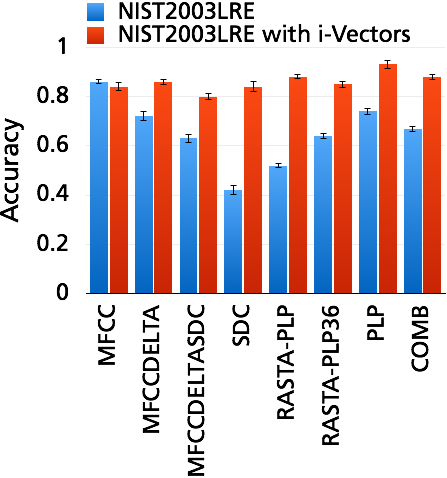
\includegraphics[width=\textwidth]{images/lid_exp1a_nist.png}
                \caption{NIST2003LRE}
                \label{fig:lid_exp1a_nist}
        \end{subfigure}%
        \begin{subfigure}[b]{0.3\textwidth}
                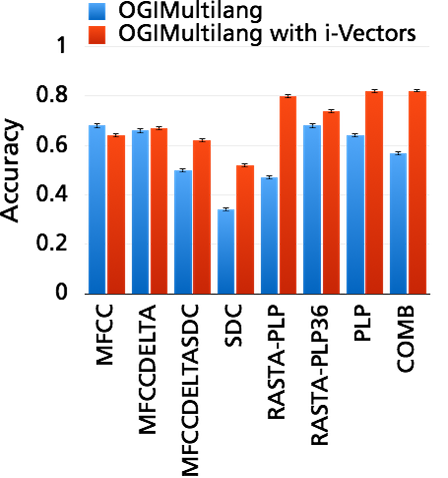
\includegraphics[width=\textwidth]{images/lid_exp1a_ogi.png}
                \caption{OGIMultilang}
                \label{fig:exp1a_ogi}
        \end{subfigure}
                \begin{subfigure}[b]{0.3\textwidth}
                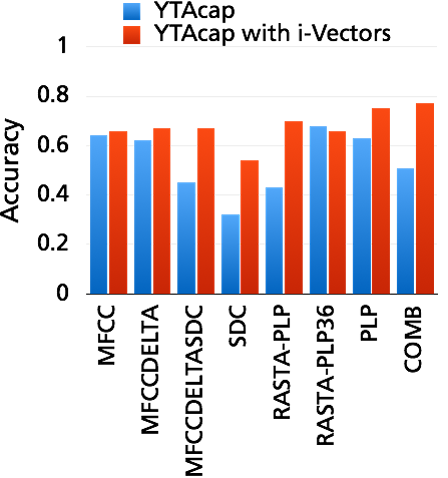
\includegraphics[width=\textwidth]{images/lid_exp1a_yt.png}
                \caption{YTAcap}
                \label{fig:exp1a_yt}
        \end{subfigure}
        \caption{Results using SVM models on all three language identification data sets, with or without i-vector processing, with speakers shared between training and test sets.}\label{fig:lid_exp1a}
\end{figure}


Figure \ref{fig:lid_exp1a} shows the results for the SVM models trained on the same data sets. In general, these models appear to be able to capture the language boundaries better.\\
In contrast to the MLP experiment, SVMs produced good results on the \textit{NIST2003LRE} data set for all of the features. They seem to be able to discriminate very well on this small, clean data set. The best result with i-vector processing is $86\%$ for MFCC features. When using i-vectors, 93\% are achieved with PLP features. This may, in fact, be close to the upper bound for the classification here, which might be caused by annotation errors or ambiguous data.\\
The \textit{OGIMultilang} corpus is bigger and more varied than the \textit{NIST2003LRE} corpus, which makes it harder to classify. As shown, the high-dimensional pure features did not perform as well, with a maximum of 68\% for MFCCs and RASTA-PLPs with 36 coefficients. Using i-vector extraction improved the result by a large margin. Feature-wise, PLPs without RASTA processing seem to work best at a result of 82\%. 
%CHECK!!!
MFCC and SDC features did not work quite as well, but did not hurt the result either when combined with PLPs (COMB result). It is interesting to see that the i-vector extraction decreased the results for MFCCs, the feature that worked best without it.\\
%CHECK!!
Similar to the \textit{OGIMultilang} corpus, the \textit{YTAcap} corpus provides very complex and varied data. The same effects occur on the direct feature training here, too: RASTA-PLPs with 36 coefficients provide the best results, but the accuracy is not very high at 68\%. i-vector extraction once again serves to improve the result. The highest results when using i-vector extraction are 75\% when using PLP without RASTA processing or 77\% for the COMB configuration.

\subsection{Experiments with unknown speakers}

In order to find out what influence the speaker characteristics had on the result, the same experiments were then repeated with training and evaluation sets that strictly separated speakers. This experiment was not performed for the \textit{NIST2003LRE}�corpus because no speaker information is available for it. Since the SVM models performed much better in the previous experiment, only these models were tested.\\

\begin{figure}[h]
       \centering
      %\begin{subfigure}[b]{0.3\textwidth}
        %        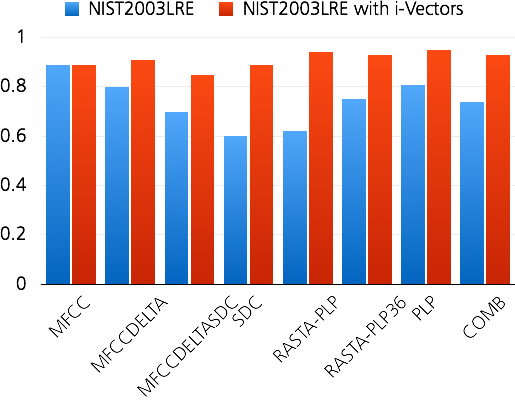
\includegraphics[width=\textwidth]{images/lid_exp2_nist.png}
         %      \caption{NIST2003LRE}
           %     \label{fig:lid_exp2_nist}
        %\end{subfigure}%
        \begin{subfigure}[b]{0.4\textwidth}
                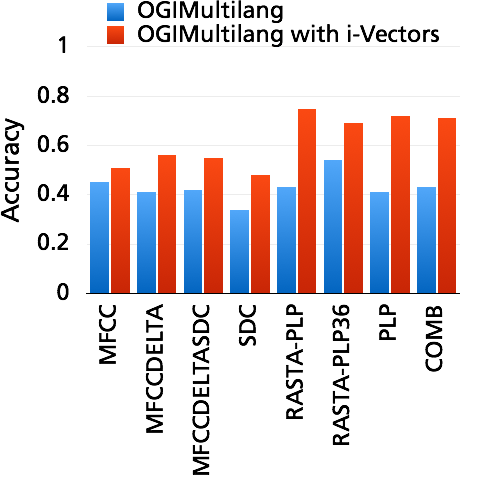
\includegraphics[width=\textwidth]{images/lid_exp2_ogi.png}
                \caption{OGIMultilang}
                \label{fig:exp2_ogi}
        \end{subfigure}
                \begin{subfigure}[b]{0.4\textwidth}
                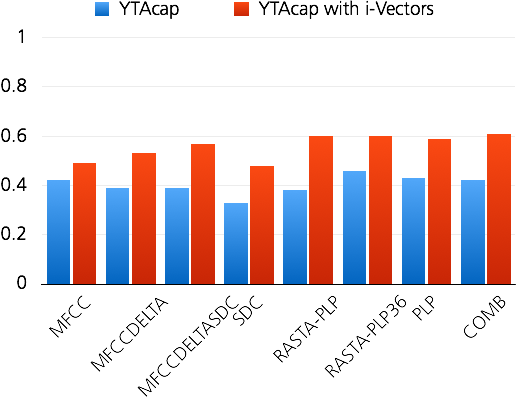
\includegraphics[width=\textwidth]{images/lid_exp2_yt.png}
                \caption{YTAcap}
                \label{fig:exp2_yt}
        \end{subfigure}
        \caption{Results using SVM models on all three language identification data sets, with or without i-vector processing, with speakers separated between training and test sets.}\label{fig:lid_exp2}
\end{figure}

The results are shown in figure \ref{fig:lid_exp2}. In general, all configurations performed worse, indicating that some of the characteristics learned by the models come from the speakers rather than the languages. Apart from this, the general trends for the features remain the same, and i-vector extraction still improves the over-all results.\\

On the \textit{OGIMultilang} corpus, the best result is still obtained with RASTA-PLP features and i-vector processing, but the accuracy falls by around 8 percent points to $75\%$. On \textit{YTAcap}, the effect is even worse: From an accuracy of $77\%$ with the mixed condition, the result decreases to $61\%$ for the separated condition. The reason for this is probably the wider signal variety in singing as opposed to speech; additionally, \textit{YTAcap} also possesses a wider range of recording conditions than the controlled telephone conditions of \textit{OGIMultilang}. Arguably, the solution for this effect would be the use of larger training data sets, which would be able to cover these acoustic and performance conditions better. Conversely, as the previous results show, the approach functions better when an application scenario can be limited to a range of known speakers, or at least recording conditions (as in the \textit{NIST2003LRE} experiment).


%TODO: info about speakers and material per speaker
\subsection{Experiments with utterances combined by speakers}

All previous experiments were performed on relatively short utterances of a few seconds in duration. In many application scenarios, much more audio data is available to make a decision about the language. In particular, songs are usually a few minutes in length, and in many cases, only one result per document (=song) is required.\\
For this reason, results for the \textit{YTAcap} data set were taken from the previous experiment and summed up for each song (and therefore also for each singer). For the \textit{OGIMultilang} corpus, results for all utterances by the same speaker were aggregated in the same fashion, resulting in similar durations of audio. (Again, this experiment was not performed with the \textit{NIST2003LRE} corpus due to the lack of speaker information).\\

\begin{figure}[h]
       \centering
           \begin{subfigure}[b]{0.4\textwidth}
                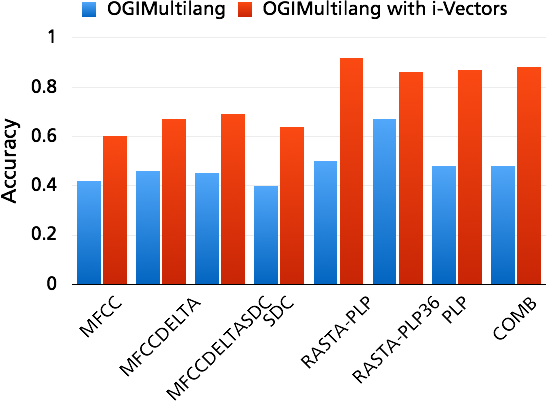
\includegraphics[width=\textwidth]{images/lid_exp3_ogi.png}
                \caption{OGIMultilang}
                \label{fig:exp3_ogi}
        \end{subfigure}
                \begin{subfigure}[b]{0.4\textwidth}
                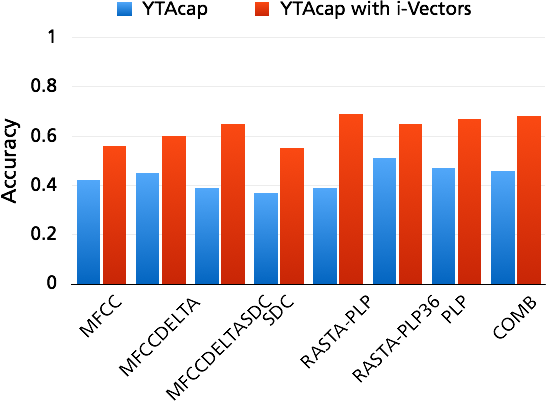
\includegraphics[width=\textwidth]{images/lid_exp3_yt.png}
                \caption{YTAcap}
                \label{fig:exp3_yt}
        \end{subfigure}
        \caption{Document-wise results using SVM models, with or without i-vector processing.}\label{fig:lid_exp3}
\end{figure}

The results are shown in figure \ref{fig:lid_exp3}. Overall, aggregation of multiple utterances by the same speakers seems to balance out some of the speaker-specific effects seen in the previous experiment. Taking more acoustic information into account, the models are able to determine the language with higher accuracy.\\
On the \textit{OGIMultilang} corpus, the result is even better than on the condition with known speakers. The best result rises from $75\%$ for short utterances to $92\%$ for the aggregated documents (both with the RASTA-PLP feature). On the \textit{YTAcap} data sets, the aggregated result is $69\%$ (compared to $60\%$ for line segments).\\

As suggested in the previous section, the approach produces practically usable results when the problem can be narrowed down, e.g. to known speakers or recording conditions. As this experiment shows, useful results can also be obtained when longer sequences are available for analysis. 


\

%nicht n�tig f�r nist - kleine datenmengen gehen so mit svm. bei mlp aber overfitting.
%ogi: ivec erh�ht Ergebnis massiv. besser als irmfsp (warum?)
%yt: �hnlich ogi. Ergebnisse > sota. 
%features: plp gut, am besten ohne Rasta (warum?). mehr coeffs bringen aber nichts. mfcc f�r sich auch gut, mit delta noch besser, teilweise auch mit sdc.
%combi aus plp_norasta und mfccdelta funktioniert am besten - 2 verschiedene Aspekte abgedeckt (warum?)
%insgesamt: schnelleres training und weniger Speicherplatz als volle features, Irrelevanz reduziert. �hnliche Ergebnisse wie pprlm, aber viel einfacher. weniger Annotationen und leichter zu implementieren.




\section{LID in singing using phoneme recognition posteriors}
Another developed approach is based upon phoneme statistics derived from phoneme posteriorgrams. To obtain representative statistics for model training, relatively long observations are necessary, but, as described in the previous section, this is the case for many applications, for example when considering song material (e.g. songs of 3-4 minutes in duration). On the other hand, phoneme posteriorgrams need to be calculated for a number of other tasks, such as keyword spotting or lyrics-to-audio alignment. \\

\begin{figure*}
	\begin{center}
		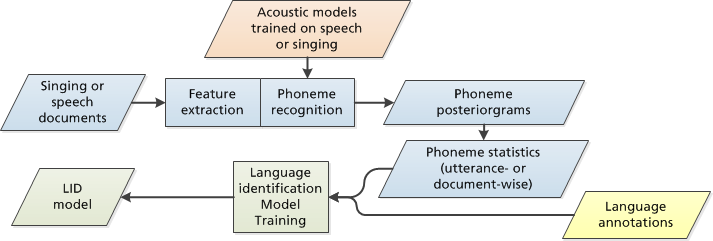
\includegraphics[width=.8\textwidth]{images/lid_statistics_process.png}
		\caption{Overview of the process for language identification using phoneme statistics.}
		\label{fig:lid_statistics_process}
	\end{center}
\end{figure*}

An overview of the approach is shown in figure \ref{fig:lid_statistics_process}. Posteriorgrams were generated on the test data sets \textit{YTAcap} and \textit{OGIMultilang} using the acoustic models trained on the \textit{TIMIT} speech data set and on the \textit{DAMP} singing data set as described in section \ref{sec:phonerec_acap}. To facilitate the following language identification, phoneme statistics were then calculated in two different ways:
\begin{description}
 \item[Utterance-wise statistics]{Means and variances of the phoneme likelihoods over each utterance were calculated (or, in the case of \textit{YTAcap}, over each song segment). For further training, the resulting vectors for each speaker/song (=document) were used as a combined feature matrix. As a result, no overlap of speakers/songs was possible between the training and test sets.}
 \item[Document-wise statistics]{Mean and variances of the phoneme likelihoods over whole songs or sets of utterances of a single speaker were calculated. This resulted in just two feature vectors per document (one for the means, one for the variances).}
\end{description}
Naturally, relatively long recordings are necessary to produce salient statistics. For this reason, the aggregation by speaker/song was done in both cases rather than treating each utterance separately. \\

Then, Support Vector Machine (SVM) models were trained on the calculated statistics in both variants with the three languages as annotations. Unknown song/speaker documents could then be subjected to the whole process and classified by language.\\
Again, all results in the were obtained using 5-fold cross-validation - i.e., SVMs were trained on 4/5 of each corpus, then the remaining 1/5 was classified with the model. This was done 5 times until each song/speaker document had been classified.

\subsection{Language identification using document-wise phoneme statistics}
In the first experiments, SVM classifiers were trained on the document-wise phoneme statistics, and classification was also performed on a document-wise basis (i.e., only one mean and one variance vector per document). The results are shown in figure \ref{fig:lid_statistics_res1} in terms of accuracy (average retrieval when all documents are classified into exactly one language).\\
On the singing test set, results are worst when using acoustic models trained on \textit{TIMIT} at just $53\%$ accuracy, and become better when using the model trained on the \textit{TIMIT} variant modified for singing or the small selection of the singing training set ($59\%$ each). The best result is achieved when the models are trained on the full singing data set at $63\%$ accuracy.\\
Surprisingly, the results on the \textit{OGIMultilang} corpus also improve from $75\%$ with the \textit{TIMIT} models to $84\%$ using the \textit{DampB} models. Since \textit{TIMIT} is a very ``clean'' data set, training on the song corpus might provide some more phonetic variety, acting as a sort of data augmentation. This could be especially important in this context where phonemes are recognized in three different languages.\\
On both corpora, there is no noticeable bias of the confusion matrix - i.e., the confusions are spread out evenly. This is particularly interesting when considering that the acoustic models were trained on English speech or singing only.
%\begin{figure}[h]
 %       \centering
  %      \begin{subfigure}[b]{0.25\textwidth}
  %              \includegraphics[width=\textwidth]%{figs/stat_acc.png}
   %             \caption{Accuracy}
   %             \label{fig:stat_acc}
  %      \end{subfigure}%
   %     ~ %add desired spacing between images, e. g. ~, \quad, \qquad, \hfill etc.
          %(or a blank line to force the subfigure onto a new line)
   %     \begin{subfigure}[b]{0.25\textwidth}
     %           \includegraphics[width=\textwidth]%{figs/stat_cavg.png}
   %             \caption{Average cost}
  %              \label{fig:stat_cavg}
 %       \end{subfigure}
 %       \caption{Results using document-wise phoneme statistics generated with various acoustic models.}\label{fig:res_stat}
%\end{figure}

\begin{figure*}
	\begin{center}
		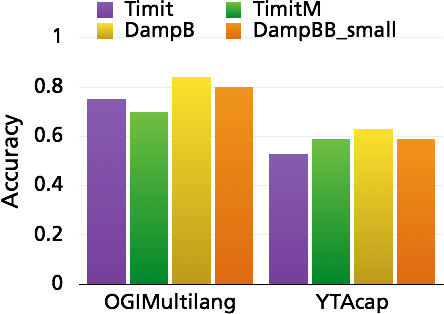
\includegraphics[width=.5\textwidth]{images/lid_statistics_res1.png}
		\caption{Results using document-wise phoneme statistics generated with various acoustic models.}
		\label{fig:lid_statistics_res1}
	\end{center}
\end{figure*}

\subsection{Language identification using utterance-wise phoneme statistics}
Next, language identification was performed with models trained on the statistics of each utterance contained in the document. The recognition process is still performed on the whole document. The results are reported in figure \ref{fig:lid_statistics_res2}.\\
Phoneme statistics may not be as representative when computed on shorter inputs, but they may provide more information for the backend model training when utilized as a combined feature matrix for a longer document. The results on singing improve slightly to $63\%$ with the acoustic model trained on the small singing corpus (\textit{DampBB\_small}) and decrease slightly for the \textit{DampB} model ($61\%$). However, on the speech corpus, the best result rises to $90\%$.
%why??
%\setlength{\belowcaptionskip}{-0.3cm}
%\begin{figure}[h]
 %       \centering
 %       \begin{subfigure}[b]{0.25\textwidth}
  %              \includegraphics[width=\textwidth]%{figs/stats_acc.png}
  %              \caption{Accuracy}
 %               \label{fig:stats_acc}
%        \end{subfigure}%
 %       ~ %add desired spacing between images, e. g. ~, \quad, \qquad, \hfill etc.
          %(or a blank line to force the subfigure onto a new line)
 %       \begin{subfigure}[b]{0.25\textwidth}
 %               \includegraphics[width=\textwidth]%{figs/stats_cavg.png}
 %               \caption{Average cost}
  %              \label{fig:stats_cavg}
  %      \end{subfigure}
  %      \caption{Results using utterance-wise phoneme statistics generated with various acoustic models.}\label{fig:res_stats}
%\end{figure}
%\setlength{\belowcaptionskip}{-0.1cm}
\begin{figure*}
	\begin{center}
		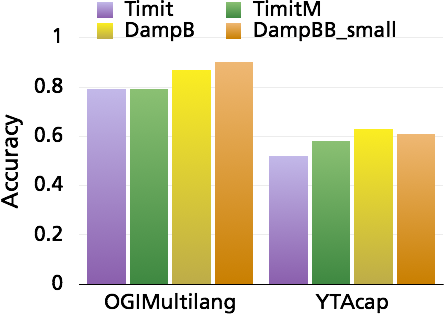
\includegraphics[width=.5\textwidth]{images/lid_statistics_res2.png}
		\caption{Results using utterance-wise phoneme statistics generated with various acoustic models.}
		\label{fig:lid_statistics_res2}
	\end{center}
\end{figure*}

\subsection{For comparison: Results for the i-vector approach}
For comparison, models from the previous approach were also trained on the same time scales. I-vectors were calculated on the utterance- or the document-wise scale. This was done for PLP and MFCC features. The resulting i-vectors were then used to train SVMs in the same manner as in the previous experiments. (The difference here is that the models are already trained on the aggregated i-vectors, either with those for a whole document or with all i-vectors of the utterances constituting each document aggregated). The results are shown in figure \ref{fig:lid_statistics_res3}.\\
The best result obtained on \textit{YTAcap} corpus is $68\%$ accuracy. This is only 5 percent points higher than the presented approach, which is much easier to implement. On the \textit{OGIMultilang} data set, the difference is only 3 percent points ($93\%$). Of course, the advantage of the i-vector approach is that it can also be performed on much shorter inputs.\\

\begin{figure*}
	\begin{center}
		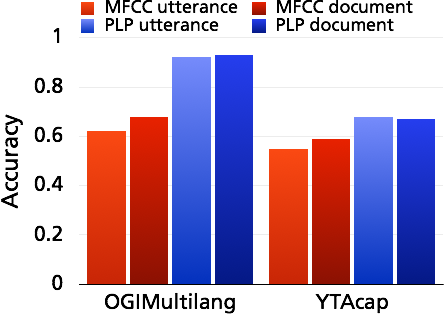
\includegraphics[width=.5\textwidth]{images/lid_statistics_res3.png}
		\caption{Results using utterance- and document-wise i-vectors calculated on PLP and MFCC features.}
		\label{fig:lid_statistics_res3}
	\end{center}
\end{figure*}
%\begin{figure}[h]
 %       \centering
%        \begin{subfigure}[b]{0.25\textwidth}
 %               \includegraphics[width=\textwidth]%{figs/ivec_acc.png}
  %              \caption{Accuracy}
   %             \label{fig:ivec_acc}
  %      \end{subfigure}%
  %      ~ %add desired spacing between images, e. g. ~, \quad, \qquad, \hfill etc.
          %(or a blank line to force the subfigure onto a new line)
 %       \begin{subfigure}[b]{0.25\textwidth}
 %               \includegraphics[width=\textwidth]%{figs/ivec_cavg.png}
 %               \caption{Average cost}
  %              \label{fig:ivec_cavg}
  %      \end{subfigure}
  %      \caption{Results using utterance- and document-wise i-vectors calculated on PLP and MFCC features.}\label{fig:res_ivec}
%\end{figure}

\section{Conclusion}\label{sec:lid_conclusion}
In this section, two approaches to singing language identification were presented: One based on i-vector processing of audio features, and one based on phoneme statistics generated from posteriorgrams. In both cases, machine learning models were trained on the resulting data.\\

In the first approach, PLP, MFCC, and SDC features were extracted from audio data, and then run through an i-vector extractor. The generated i-vectors were then used as inputs for MLP and SVM training. The basic idea behind the i-vector approach is the removal of speaker- and channel-dependent components of the signal. This effectively reduces irrelevance to the language identification tasks and also reduces the amount of training data massively.\\
The smallest data set is the \textit{NIST2003LRE} corpus. No feature configuration achieved good results when using the MLP backend. In this case, the small size of the corpus may lead to overtraining. I-vector processing only amplified this problem by reducing the amount of data even further. The SVM backend, however, produced good results of up to 93\% for PLP features with i-vector extraction.\\
The \textit{OGIMultilang} corpus is a much bigger speech corpus. Training without i-vector extraction did not work well for any feature configuration. The best accuracy for this scenario was 68\%. Results of up to 83\% were achieved with i-vector processing. There does not seem to be a large difference between SVM and MLP training, with SVM having just a slight advantage.\\
Language identification for singing was expected to be a harder task than for speech due to the factors described in section \ref{sec:sota_speechtosinging}. The results on the \textit{YTAcap} corpus turned out to be somewhat worse than those for the \textit{OGIMultilang} corpus, which is of similar size. As on \textit{OGIMultilang}, i-vector extraction improved the results. In this case, the accuracy improved from 63\% to 73\%.\\
The same experiment was performed again, this time with no speaker overlap between training and test sets. The results fell significantly, indicating speaker influence on the model training. In a third experiment, the results were aggregated into documents by each speaker, which again led to improved results. The best accuracy on \textit{OGIMultilang} is $92\%$, while on \textit{YTAcap}, it is $69\%$. Both experiments demonstrate that useful results can be obtained when limiting the task, e.g. by training on a set of known speakers or recording conditions, or by analyzing documents of longer durations. Alternatively, a wider range of speakers in the training data could lead to models that generalize better.\\
Overall, i-vector extraction reduces irrelevance in the training data and there leads to a more effective training. As additional benefits, the training process itself is much faster and less memory is used due to its data reduction properties. Most of the state-of-the-art approaches are based on PPRLM, which requires phoneme-wise annotations and a highly complex recognition system, using both acoustic and language models. In this respect, this system is easier to implement and merely requires language annotations.\\

The second presented method is a completely new language identification approach for singing. It is based on the output of various acoustic models, from which statistics were generated and SVM models were trained. In contrast to similar approaches for speech, no voice tokenization is performed. Since phoneme recognition on singing is not always reliable, the statistics are calculated directly on the phoneme posteriorgrams, although this does not take any temporal information into account. The acoustic models were trained only on English-language material (speech and singing); it would be interesting to test this with multi-language training data. Due to the statistics-based nature of the approach, it is not suited for language identification of very short audio recordings.\\
The accuracy of the result for singing is somewhat worse than the results obtained with the i-vector based approach. However, this new approach is much easier to implement and the feature vectors are shorter. For many applications, such posteriors need to be extracted anyway and can then efficiently be used for language identification when long observations are available. The best accuracy of $63\%$ is obtained with acoustic models trained on the \textit{DampB} singing corpus.\\
Interestingly, the best result on the \textit{OGIMultilang} speech corpus is also obtained with these acoustic models (and is only 3 percent points below the one obtained with the i-vector approach). This possibly happens because the singing corpora provide a wider range of phoneme articulations. It would be interesting to try out these acoustic models for other phoneme recognition tasks on speech where robustness to varied pronunciations is a concern.



